\documentclass[../report.tex]{subfiles}

	\subsection{Symbolic Aggregate Approximation (SAX)} \label{sec:paasax}
	SAX (\textbf{S}ymbolic \textbf{A}ggregate appro\textbf{X}imation) \citep{sax} is a technique where by a single dimension of a time series is reduced to a string of symbols for pattern matching.  The technique involves first transforming the normalised time-series in to a Piecewise Aggregate Approximation (\textbf{PAA}) which is then represented by a fixed number of symbols.  The normalisation technique is \textit{Z-normalisation} which is discussed in \cref{sec:Z-normalisation}.
	
	For the PAA, the data is first divided into equal sized time frames (see diagram below), then the mean deviation from zero of each frame is calculated.  An appropriate number of breakpoints symmetrical along the x-axis are created so that they follow a Gaussian distribution and a symbol assigned to each range between the breakpoints.  Then for each frame, a symbol is assigned based on which range the mean falls in to.  The symbols assigned to each frame are then concatenated in to a string and it is this string that gives the SAX representation of that data.  The width of the time frame and the number of discrete regions would be two parameters passed to this process alongside the data.
	\begin{figure}[h]
		\begin{subfigure}{0.5\linewidth}
			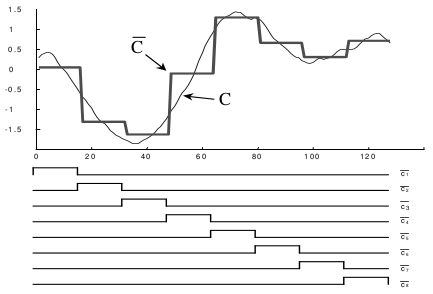
\includegraphics[scale=0.5]{paa.png}
			\caption{Calculating PAA}
		\end{subfigure}
		\begin{subfigure}{0.5\linewidth}
			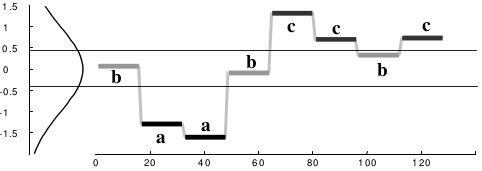
\includegraphics[scale=0.5]{sax.png}
			\caption{Diagrams showing PAA to SAX on a time-series (taken from \cite{sax})}
		\end{subfigure}
	\end{figure}